%\chapter{Introduction}



% A TOP DOWN APPROACH 
\chapter{Real number representations: a review}\label{chap:real_reps}

\lettrine{D}{ealing} with machine learning, linear algebra applications or whichever scientific task requires the use of real numbers. Mathematically speaking, a real number $r \in \mathbb{R}$, belongs to a continuous space. In a digital domain, where quantities are \textit{discrete}, we need to fall back to a discrete space to represent such numbers.  In particular, we rely on the subset of \textit{rational} numbers $\mathbb{Q} \subseteq \mathbb{R}$.

Theoretically, we could represent any rational number $q \in \mathbb{Q}$ using a couple of integer numbers $n,d \in \mathbb{Z}$ such that $\frac{n}{d} = q$. Therefore, all the operations involved between such numbers would be operations between integers, that are discrete quantities. In practice, we typically resort to a subset $\mathbb{X} \subseteq \mathbb{Q}$, where the different format representations lie.

\begin{figure}
    \centering
    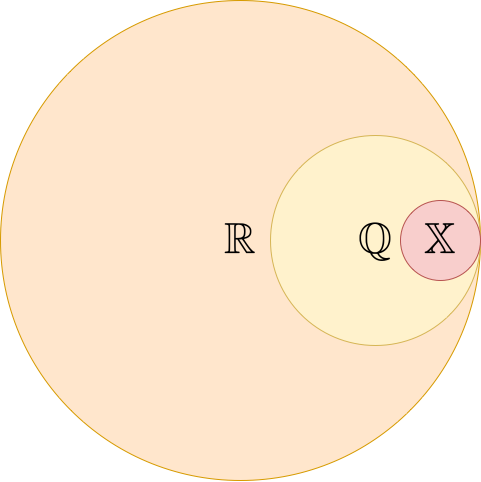
\includegraphics[width=0.3\linewidth]{img/real_sets.png}
    \caption{Visualization of real and rational number sets. $\mathbb{X}$ is the subset covered by a given format representation.}
    \label{fig:my_label}
\end{figure}

Hereafter, we will cover several real number representations, starting from the IEEE standards.


\section{The IEEE 754 Floating Point standard}

The IEEE 754 standard for floating point \cite{893287} defines a floating-point value as a 32, 64 or 128-bit fixed-size format with three fields:
\begin{itemize}
    \item Sign (always on 1-bit) $s$
    \item Exponent $e$ (as signed integer) on $E$ bits
    \item Numerator of the fractional part of the mantissa $f$ (as an unsigned integer) on $F$ bits
\end{itemize}

The real value $r$ associated with a given float representation is the following:

\begin{equation}\label{eqn:float2real}
    r = (-1)^s \cdot 2^{e-k} \cdot (1.f)
\end{equation}

The expression $1.f$ is a shorthand for the mantissa $m = 1 + \frac{f}{2^F} \in [1,2) \subseteq \mathbb{Q}$.

The constant value $k$ is a \textit{bias} applied to the exponent for normalization purposes. The bias value is computed as follows: $k = 2^{E-1}$ - $1$.



\begin{table}[b]
\centering
\caption{Bit configuration for different IEEE754 floats}
\label{tab:ieee754configs}
\begin{tabular}{l|lll}
\hline
          & Exponent bits & Bias  & Fraction bits \\ \hline
binary16 (half) &  5             & 15    & 10            \\ \hline
binary32 (single) & 8             & 127   & 23            \\ \hline
binary64 (double) & 11            & 1023  & 52            \\ \hline
binary128 (quad) & 15            & 16383 & 112           \\ \hline
\end{tabular}
\end{table}

The four different IEEE 754 configurations are called, respectively: binary16 (half-precision), \\binary32 (single-precision), binary64 (double-precision) and binary128 (quadruple-precision). Table \ref{tab:ieee754configs} summarizes the different bit configurations for the four formats.

Besides the \textit{normal} representation, there are \textit{special} bit patterns that represent special numbers:
\begin{itemize}
    \item $e = 0$ and $f \neq 0$: subnormal numbers
    \item $e = 2^{E} - 1$ and $f = 0$: infinity
    \item $e = 2^{E} - 1$ and $f \neq 0$: not a real/not a number
\end{itemize}

Subnormals are a class of numbers that fill the gap of real representations between zero and the minimum normal number (in absolute value). When the exponent $e$ is $0$ and the fraction is non-zero the exponent value in Equation \ref{eqn:float2real} is set to $2^{-k+1}$ and the leading $1$ in the mantissa part is removed (0.f instead of 1.f), with $0.f \in [0,1) \subseteq \mathbb{Q}$

A particular mention goes to the representation for the real value $0$, which can be either positive or negative, having two representations.


\section{The Fixed Point representation}

Unlike floating point formats, the fixed point representation has a predefined amount of digits for the decimal part. Fixed point numbers are stored as plain integers with implicit scaling factors (e.g. the value $0.50$ can be stored as $50$ with an implicit scaling factor of 100).

Generally, a $N$-bit fixed point format has three \textit{fields}:

\begin{itemize}
    \item Sign $s$ on $1$ bit
    \item Integral part $i$ (as unsigned integer) on $I = \frac{N}{2} - 1$ bits
    \item Fractional part $f$ (as unsigned integer) on $F = \frac{N}{2}$ bit
\end{itemize}

The real value $r$ represented by a given fixed point in this format is:
\begin{equation}\label{eqn:fixed2real}
    r = (-1)^s \cdot \left( i + 0.f \right)
\end{equation}

Note that we can see the term $0.f$ in \eqref{eqn:fixed2real} as:
\[
    \sum_k^F f_k \cdot 2^{-k} = \frac{f}{2^F}
\]

Where $f_k$ is the k-th bit of the integer $f$.

As an example, we report the representation of the real number $6.25$ for a 16-bit fixed-point format.

Such format has a 7-bit integral part, that can be represented as $(6)_{10} = {(0000110)}_{2}$.
The fractional part is on 8 bits and can be represented as $ .(25)_{10} = .(0100000)_{2}$

Fixed point numbers are peculiar thanks to the fact that operations that involve such numbers can be implemented efficiently using integer arithmetic.

The algebraic sum of two fixed points can be represented as follows:
\begin{equation}\label{eqn:fixedSum}
    r_1 + r_2 = \left(i_1 \pm i_2 + \frac{f_1 \pm f_2}{2^{F}}\right)
\end{equation}

This is equivalent to the sum of the two fixed point representations.

Differently, the multiplication can be represented as follows:
\begin{equation}\label{eqn:fixedMul}
    r_1 \cdot r_2 = -1^{s_1 \oplus s_2}\cdot \left(i_1 \cdot i_2 + \frac{i_1 \cdot f_2 + f_1\cdot i_2 + f_1 \cdot f_2}{2^F}\right) 
\end{equation}

Where $\oplus$ is a bit-wise xor.

As we can see this is not directly relatable to the multiplication of representations due to the cross-products between integral and fractional parts.

\section{The BFloat family: BFloat16 and BFloat8}

The Brain Float16 (BFloat16) format \cite{burgess2019bfloat} is a revision of the IEEE binary16 that modifies the number of allocated bits for the different fields:

\begin{itemize}
    \item Sign (always on 1-bit) $s$
    \item Exponent $e$ (as signed integer) on $8$ bits
    \item Fractional part of the mantissa $f$ (as an unsigned integer) on $7$ bits
\end{itemize}

The format definition stands out for the fact that it shares the same number of bits for the exponent as binary32 does. Therefore, the exponent offset is the same, $127$ and the real value $r$ associated with a given BFloat16 is:

\begin{equation}\label{eqn:bfloat162real}
    r = (-1)^s \cdot 2^{e-127} \cdot \left(1 + \frac{f}{2^7} \right)
\end{equation}

Thanks to its similarity to the binary32 format, the BFloat16 can be seen as a truncated version of the former. This means that the conversion between the two formats is just a matter of shifting 16 positions left or right.

The Brain Float8 (BFloat8) format \cite{naveen2019mixed} is a further compression of the binary16 format, with the following fields:

\begin{itemize}
    \item Sign (always on 1-bit) $s$
    \item Exponent $e$ (as signed integer) on $5$ bits
    \item Fractional part of the mantissa $f$ (as unsigned integer) on $2$ bits
\end{itemize}

The format definition highlights the similarity with binary16, having the same number of exponent bits (hence, the same exponent offset). The real value $r$ associated to a given BFloat8 is:

\begin{equation}\label{eqn:bfloat82real}
    r = (-1)^s \cdot 2^{e-15} \cdot \left(1 + \frac{f}{2^2} \right)
\end{equation}

Since it shares the same number of exponent bits with binary16, the conversion between the two formats is just a matter of shifting 8 positions left or right.

The authors of \cite{naveen2019mixed} also introduced the concept of \textit{stochastic rounding}, mainly used during the training of neural networks.

Suppose we want to round a floating point number $x$, with $s,e,m$ being, respectively, sign, exponent and mantissa $m$ (where $m = 1 + frac$). The fractional part $frac$ is originally represented on $k'$ bits and needs to be truncated into $\lfloor m \rfloor$ on $k$ bits. Let us define the probability: 
\begin{equation}\label{eqn:bfloat8StochProb}
    p = \frac{frac- \lfloor frac \rfloor}{\epsilon}
\end{equation}

where $\epsilon = 2^{-k}$.

Following the \textit{stochastic rounding approach}, the rounded value of $x$ will be:
\begin{equation}\label{eqn:bfloat8Rounded}
\text{Round}(x) = 
\left\{\begin{matrix}
s \cdot 2^e \cdot ( 1 + \lfloor frac \rfloor + \epsilon) & \text{with probability } p \\ 
s \cdot 2^e \cdot ( 1 + \lfloor frac \rfloor) & \text{with probability } 1-p 
\end{matrix}\right.
\end{equation}

\section{Flexpoint}
The Flexpoint format \cite{koster2017flexpoint,popescu2018flexpoint} combines fixed and floating point arithmetic. In particular, given a tensor $T$, all the values inside it are represented with a shared exponent. Each of these values is represented as a fixed-point with $N$-bits mantissa. All the values then share a common exponent on $M$ bits. The authors call such a format $\text{flex}N+M$; the counterpart for a binary32 number is $\text{flex}16+5$, according to the authors.

Thanks to this approach, the memory footprint of tensors is heavily reduced and, consequently, the bandwidth required by the hardware is reduced. In particular, if we employ GPU computing, we only need to transfer an integral part to the device while the shared exponent can be left on the host domain. 

The authors also propose automatic exponent management, which adjusts the exponent scale according to historical predictions of exponent changes. In particular, if the dataset contains independent and identically distributed samples, we can expect exponent values to change slowly during training epochs.

\section{Logarithmic Number System (LNS)}

The Logarithmic Number System \cite{johnson2018rethink} is a system where any number $X$ is represented as follows:
\begin{equation}\label{eqn:logNumSysSet}
    X \xrightarrow[]{}\{ s,x = \log_b(\left| X \right|) \}
\end{equation}

Where $b$ is the logarithm base and $s$ is the sign of the number $X$. The value $x$ is typically represented as an integer in two's complement format.

The first property that stands out from this representation is that division, multiplication and exponentiation can be transformed as follow:
\begin{equation}
    X\cdot Y \xrightarrow[]{} (s_x \oplus s_y)\cdot \left[ \log_b(X \cdot Y) \right] = (s_x \oplus s_y)\cdot \left[ \log_b(X) +  \log_b(Y) \right] = (s_x \oplus s_y)\cdot \left[ x+y \right]
\end{equation}

\begin{equation}
    \frac{X}{Y} \xrightarrow[]{} (s_x \oplus s_y)\cdot \left[ \log_b\left(\frac{X}{Y}\right) \right] = (s_x \oplus s_y)\cdot \left[ \log_b(X) -  \log_b(Y) \right] = (s_x \oplus s_y)\cdot \left[ x-y \right]
\end{equation}

\begin{equation}
    X^Y \xrightarrow[]{} \left[ \log_b(X ^ Y) \right] = (s_x \oplus s_y)\cdot \left[Y \cdot  \log_b(X)  \right] = Y\cdot x
\end{equation}

However, addition and subtraction operations are more complicated to represent. In particular, we need to employ natural logarithms:
\begin{equation}
    s_b(z) = \log_b (1 + b^z)
\end{equation}
\begin{equation}
    d_b(z) = \log_b (\left | 1 - b^z \right |)
\end{equation}

Using that two definitions we can define the sum and subtraction operations as follows:
\begin{equation}
    \log_b(|X + Y|) = x + s_b(y - x) 
\end{equation}

\begin{equation}
    \log_b(|X + Y|) = x + d_b(y - x) 
\end{equation}

%\chapter{Real number representations: a review}


